\section{Durchführung}
\label{sec:Durchfuehrung}

\begin{figure}
	\centering
	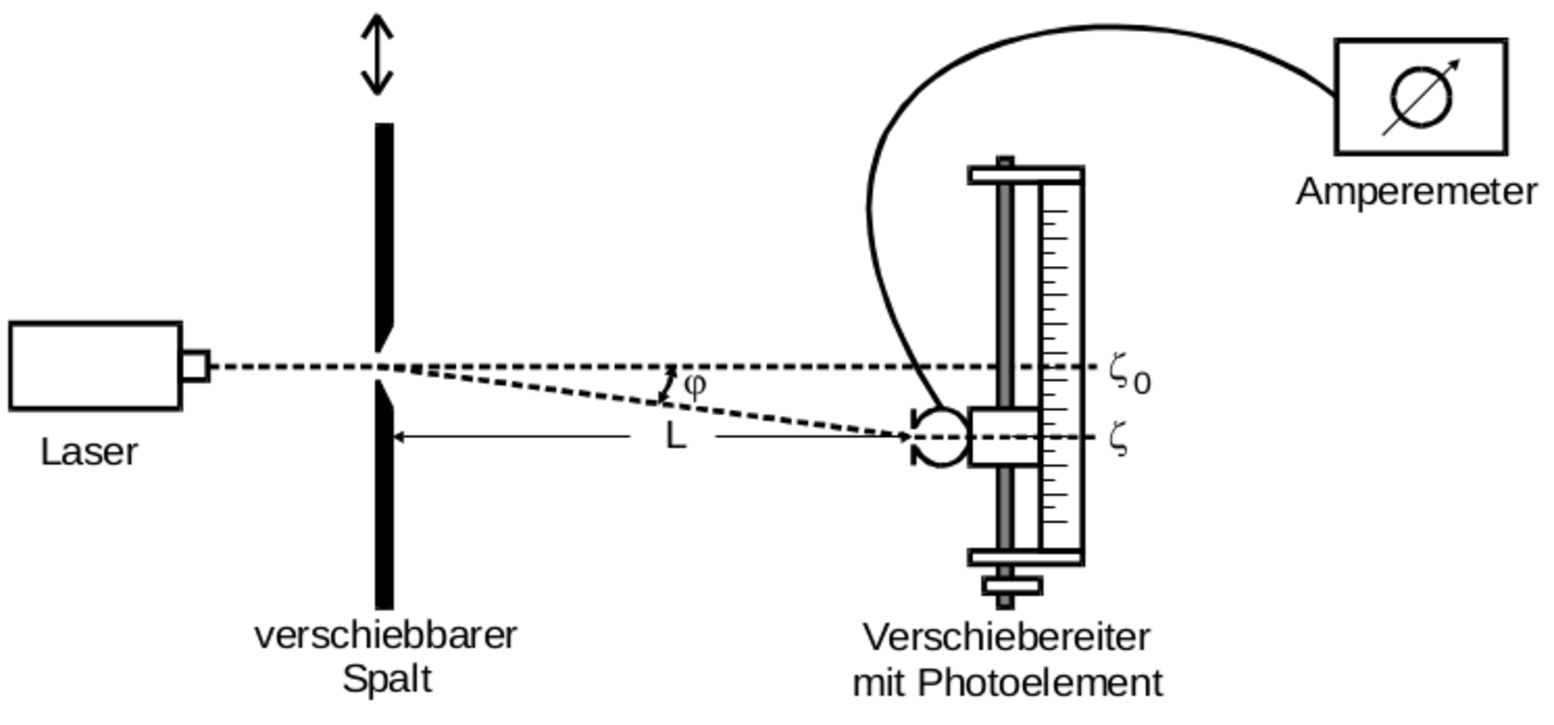
\includegraphics[width=0.7\textwidth]{Bilder/Aufbau.pdf}
	\caption{Versuchsaufbau.\cite{V406}}
	\label{fig:aufbau}
\end{figure}

Die Intensität $I$ der Beugungsfigur bei Verwendung verschiedener Spaltblenden wird punktweise ausgemessen. 
Dafür wird ein Spalt wie in Abbildung \ref{fig:aufbau} von einem Laser der Wellenlänge $\lambda=\SI{633}{\nano\meter}$ beleuchtet. 
Im Abstand $L=\SI{120.3}{\centi\meter}$ vom Spalt entfernt befindet sich ein Verschiebereiter mit Photodiode. 
Die Anordnung wird so justiert, dass das Hauptmaximum des Beugungsbildes auf die Mitte des Verschiebereiters bei \\$d_0=\SI{25}{\milli\meter}$ gerichtet ist. 
Die Photodiode wird in jedem Versuchsteil über eine Skala von $\SI{50}{\milli\meter}$ in $\SI{1}{\milli\meter}$-Schritten verschoben.
Ein an die Diode angeschlossenes Amperemeter zeigt die Intensität $I$ an. 
Bei jeder Messung wird beachtet, dass die Photodiode ohne direkte Bestrahlung durch den Laser einen thermischen Dunkelstrom $I_0$ misst. Dieser wird vor jeder Messung bestimmt und in der Auswertung berücksichtigt. 

Es werden zwei unterschiedliche Einzelspalte, sowie ein Doppelspalt untersucht. 
Anschließend werden die Spaltbreiten mit einem Mikroskop ausgemessen, dessen Vergrößerung vorher mit Hilfe von Vergleichsskalen überprüft wird. 
\newpage


